\documentclass[a4paper,10pt]{article}
\usepackage{graphicx}
\usepackage[english]{babel}
\usepackage[latin1]{inputenc}
\usepackage{gensymb}
\usepackage{amsmath}

\begin{document}

  \title{Density Lab Report}

  \author{Kaleb Moreno \\ e-mail: kalebm2@uw.edu}

  \date{\today}

  \maketitle


  \newpage

  \tableofcontents

  \pagebreak
  \section*{Data Analysis}
  
  \section{Introduction}
    \subsubsection*{What was the bigger picture?}
      
      There were a lot of big picture ideas that we covered in the days leading up to this lab, and the lab itself. One of the major ideas that we explored was the discovery of Archimedes where he learned that the volume of water displaced by an object is equal to the volume of the object. This is exactly the idea that we attempted to exercise to find the mass and composition of a modern penny.
    
    \subsubsection*{What did you do in the lab?}

      The overall purpose of this lab was to determine the mass and composition of a modern penny based on the volume of water displaced in a graduated cylinder. To accomplish this goal my lab partner and I began by determining the average density of pure water over the course of three trials. We then determined the density of seawater using the same methodology as the pure water. Finally, we performed the density study of modern pennies by recording mass, volume and density over the course of three trials. This final step gave us an average density for the pennies, which then allowed us to determine the over all composition.  

    \subsubsection*{Why is this work important?}
    
      This work is important for a lot of reasons, but more generally speaking, understanding and applying the scientific method is something every society has benefited from since its discovery. After all, It is because of the great minds throughout history that we are able to enjoy long life expectancies, and modern conveniences. As it relates to modern pennies, this sort of work is important for at least two reasons. One, from the prospective of the Treasury, knowing with accuracy the composition of a penny allows you to then find the ideal composition which minimizes costs, and maximizes efficient production. Two, being able to determine the composition of something based on its density is incredible powerful. 
    \subsubsection*{What did you test and what was your key result?}

      The following are the two hypotheses that I proposed prior to the start of the lab:
      
      \begin{enumerate}
        \item I propose that seawater will be more dense than pure water because unlike pure water, seawater contains sodium making it more dense. 
        \item I propose that pennies post 1983 have a higher zinc percentage than copper, because copper is more valuable and expensive than zinc. 
      \end{enumerate} 
      
      Interestingly, the data that I gathered in this lab confirmed only one of my hypotheses. The percent composition of zinc in the penny was indeed much higher than the percent of copper. However, my other hypothesis stands in contrast to the data. It appears that the density of the seawater that I tested was lower than the density of the pure water.  
    
      \section{Part1: Determination of Water}

    Laboratory temperature: \textbf{21.0\degree C}\\
    Mass of beaker: \textbf{50g}

    \begin{table}[h!]
    \label{tab:table1}
      \renewcommand{\arraystretch}{1.5}
      \begin{tabular}{|l|c|c|c|}
        \hline
        \textbf{Data Table 1: Water} & \textbf{Trial 1} & \textbf{Trial 2} & \textbf{Trial 3}\\
        \hline
        Tared mass of water & $5.826g$ & $6.113g$ & $6.111g$ \\
        \hline
        Volume of water ($mL$) & $5.00mL$ & $5.00mL$ & $5.00mL$ \\
        \hline
        Density of water ($\frac{g}{mL}$) & $1.17\frac{g}{mL}$ & $1.22\frac{g}{mL}$ & $1.22\frac{g}{mL}$\\
        \hline
        Average density of water ($\frac{g}{mL}$) & \multicolumn{2}{l}{$1.20\frac{g}{mL}$} & \\
        \hline
      \end{tabular}
    \end{table}

    \subsubsection*{Finding the theoretical density}
      \begin{flushleft}
        \textbf{a)} Graph the density of water (y) versus temperature (x) from Reference Table I and find the line of best fit. Write the equation for the line below.\\
        \vspace{5mm}
        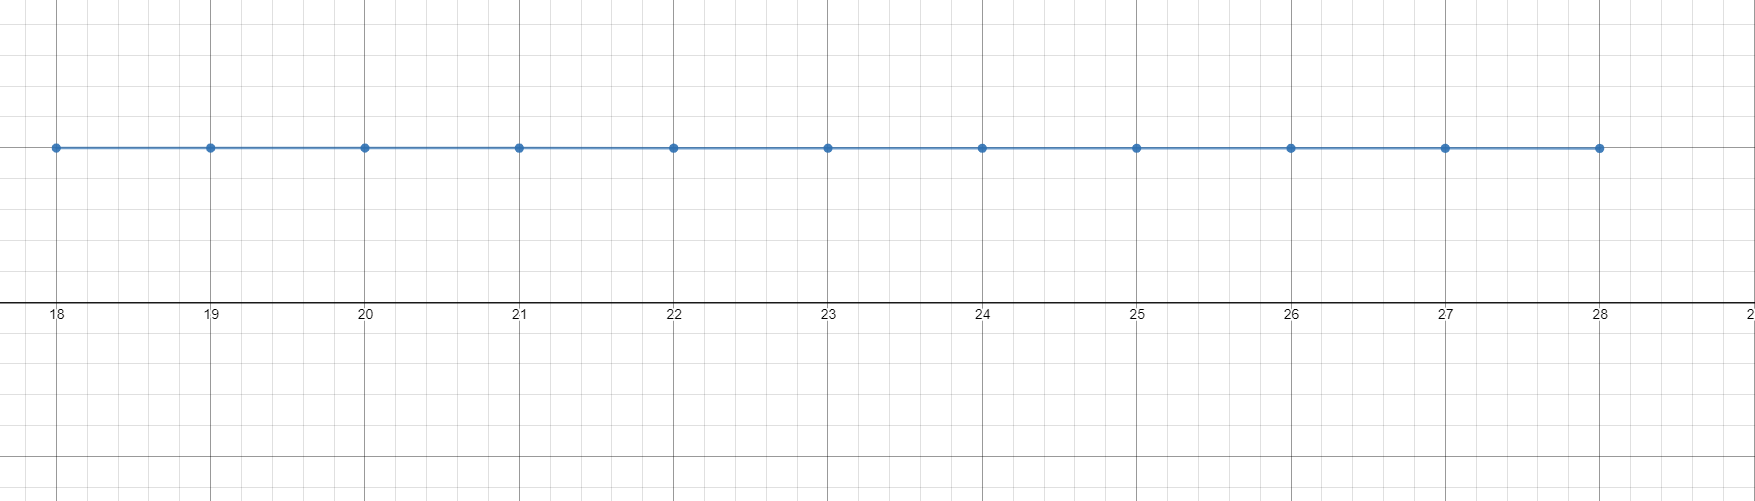
\includegraphics[width= 12cm, height= 6cm]{graph.png}
        Equation should look like:\\
        \vspace{5mm}
        $[Density] = slope * [temperature] + y-intercept$\\
        \vspace{5mm}
        $d(t) = -0.000165t + 0.00297$
        \vspace{0.25in}
        \textbf{b)} Given your line of fit, determine the theoretical density of the water given the temperature of the room. Show your calculations and your final answer. 
      \end{flushleft}

      \begin{align}
        d(21.0) &= -0.000165(21.0) + 0.00297 \\
        d(21.0) &= -0.003465 + 0.00297 \\
        d(21.0) &= -0.000495\frac{g}{mL} 
      \end{align}



  \subsubsection*{Determine the \% error of your average density of water using the theoretical density from question 2b}

  \begin{align}
    &\frac{1.20\frac{g}{mL} + 0.000495\frac{g}{mL}}{-0.000495\frac{g}{mL}} \\
    -&\frac{80033}{33}\% 
  \end{align}


  \subsubsection*{If some of the water evaporated after you added it to the beaker but before you recorded the mass, what effect would this have on your calculated density.}

    This would likely reduce the overall calculated density because water vapor is less dense than liquid water.

  \subsubsection*{Looking back at your observations, give one reason why your average density is different than the theoretical value from your answer in 2b. Your explanation must relate to your error (e.g. if your density is lower than the reported density, your explanation must explain why the density is lower).}

    One reason why my average density is perhaps different from The theoretical density, is because the theoretical density can not account for all of the variables which could impact the measurement. One such example would be the temperature of the beaker, which might offset the temperature of the water.  

  \section{Part 2: Density Determination of Seawater}

    Mass of beaker: \textbf{29.049g}

    \begin{table}[h!]
      \renewcommand{\arraystretch}{1.5}
      \label{tab:table1}
      \begin{tabular}{|l|c|c|c|}
      \hline
      \textbf{Data Table 1: Seawater} & \textbf{Trial 1} & \textbf{Trial 2} & \textbf{Trial 3}\\
      \hline
      Tared mass of seawater & $5.692g$ & $5.707g$ & $5.698g$ \\
      \hline
      Volume of seawater ($mL$) & $5.00mL$ & $5.00mL$ & $5.00mL$ \\
      \hline
      Density of seawater ($\frac{g}{mL}$) & $1.14\frac{g}{mL}$ &  $1.14\frac{g}{mL}$ & $1.14\frac{g}{mL}$ \\
      \hline
      Average density of seawater ($\frac{g}{mL}$) & \multicolumn{2}{l}{$1.14\frac{g}{mL}$} & \\
      \hline
      \end{tabular}
    \end{table}

    \subsubsection*{Using your results from Part 1 and Part 2, how many times more dense is seawater than fresh water (hint: use a ratio)? Show your calculations and give your final answer. Use equation editor for your math.}

    \subsubsection*{Considering your results, is it easier for you to float on the ocean or on a freshwater lake? Explain.}

  \section{Part 3: Determination of the Composition of a Penny through a Density Study}

  \begin{table}[h!]
    \renewcommand{\arraystretch}{1.5}
    \label{tab:table1}
    \begin{tabular}{|l|c|c|c|}
      \hline
      \textbf{Data Table 1: Penny Composition} & \textbf{Trial 1} & \textbf{Trial 2} & \textbf{Trial 3}\\
      \hline
      Number of pennies & $30$ & $35$ & $25$ \\
      \hline
      Total mass of pennies ($g$) & $81.254g$ & $93.753g$ & $68.166g$ \\
      \hline
      Initial volume of water ($mL$) & $50.8mL$ & $50.5mL$ & $50.0mL$ \\
      \hline
      Final volume of water ($mL$) & $61.0mL$ & $63.0mL$ & $59.0mL$ \\
      \hline
      Volume the pennies occupy ($mL$) & $10.2mL$ & $12.5mL$ & $9.0mL$ \\
      \hline
      Density of a penny ($\frac{g}{mL}$) & $7.97\frac{g}{mL}$ & $7.50\frac{g}{mL}$ & $7.6\frac{g}{ml}$\\
      \hline
      Average density of a penny ($\frac{g}{mL}$) & \multicolumn{2}{l}{$7.7\frac{g}{mL}$} & \\
      \hline
    \end{tabular}
  \end{table}

  \subsubsection*{Show your calculations and give your final answers for the \% zinc and \% copper in the modern penny. Use equation editor for you math.}

  \begin{align}
    8.96x\frac{g}{mL} + 7.13\frac{g}{mL} - 7.13\frac{g}{mL}x = & 7.7\frac{g}{mL} \\
    x(8.96\frac{g}{mL} - 7.13\frac{g}{mL}) + 7.13\frac{g}{mL} = & 7.7\frac{g}{mL} \\
    x(1.83\frac{g}{mL}) = & 7.7\frac{g}{mL} - 7.13\frac{g}{mL} \\
    x = & \frac{0.57\frac{g}{mL}}{1.83\frac{g}{mL}} \\
    x = & .31\frac{g}{mL} * 100 \\
    x = & 31\% \\
    x - 1 = & 69\%
  \end{align}

  \begin{flushleft}
  \textbf{Zinc: 69\%} \\
  \textbf{Copper: 31\%}
\end{flushleft}
 

  \subsubsection*{Did you need to know the exact number of pennies measured to solve for the density of a penny? Why or why not?}

    Yes, if for example you measured the mass of one penny followed by measurements of over 30 pennies, your overall average would be skewed by the single penny. however if you were given a range of 25 to 30 pennies like we were in our lab, you could calculate a fairly accurate average density without knowing the exact number of pennies. 

  \subsubsection*{Your professor will provide you with the actual composition of the modern penny. Determine the \% error for the \% zinc. Looking back at your observations, give a possible source of error from your results. Your source of error must be consistent with your observations in lab and with your results.}
    
    The percent error based on my findings, and the true density: \textbf{-29.2308\%} \\ 

    There are a number of reasons why our results did not fair well against the actual density of the modern penny. During our lab we observed the following possible sources of error: \\

   
      
    \begin{enumerate}
        \item On several occasions, the pipette created bubbles and failed to empty completely. 
        \item On our second trial measuring the density of water, we may have improperly dried the beaker.
        \item During all three trials, bubbles formed under and around the pennies as they lay stacked.
        \item The pennies never laid flat, leaving room for error.
        \item On trial 2 of measuring the density of the pennies, the pennies did not dry completely
      \end{enumerate}

  \subsubsection*{Could you reliably use the procedures and calculations in Part 3 to identify the \% composition of a nickel coin (~75~\%~Cu/~25~\% Ni)? Why or why not?}
      Given my general inaccuracy with the penny composition, I think that I personally would have a hard time identifying the \% composition of a nickel coin. I'm sure this could be done with great accuracy under the trained hands of a scientist however.  
\end{document}

